\documentclass[twoside]{book}

% Packages required by doxygen
\usepackage{fixltx2e}
\usepackage{calc}
\usepackage{doxygen}
\usepackage[export]{adjustbox} % also loads graphicx
\usepackage{graphicx}
\usepackage[utf8]{inputenc}
\usepackage{makeidx}
\usepackage{multicol}
\usepackage{multirow}
\PassOptionsToPackage{warn}{textcomp}
\usepackage{textcomp}
\usepackage[nointegrals]{wasysym}
\usepackage[table]{xcolor}

% Font selection
\usepackage[T1]{fontenc}
\usepackage[scaled=.90]{helvet}
\usepackage{courier}
\usepackage{amssymb}
\usepackage{sectsty}
\renewcommand{\familydefault}{\sfdefault}
\allsectionsfont{%
  \fontseries{bc}\selectfont%
  \color{darkgray}%
}
\renewcommand{\DoxyLabelFont}{%
  \fontseries{bc}\selectfont%
  \color{darkgray}%
}
\newcommand{\+}{\discretionary{\mbox{\scriptsize$\hookleftarrow$}}{}{}}

% Page & text layout
\usepackage{geometry}
\geometry{%
  a4paper,%
  top=2.5cm,%
  bottom=2.5cm,%
  left=2.5cm,%
  right=2.5cm%
}
\tolerance=750
\hfuzz=15pt
\hbadness=750
\setlength{\emergencystretch}{15pt}
\setlength{\parindent}{0cm}
\setlength{\parskip}{3ex plus 2ex minus 2ex}
\makeatletter
\renewcommand{\paragraph}{%
  \@startsection{paragraph}{4}{0ex}{-1.0ex}{1.0ex}{%
    \normalfont\normalsize\bfseries\SS@parafont%
  }%
}
\renewcommand{\subparagraph}{%
  \@startsection{subparagraph}{5}{0ex}{-1.0ex}{1.0ex}{%
    \normalfont\normalsize\bfseries\SS@subparafont%
  }%
}
\makeatother

% Headers & footers
\usepackage{fancyhdr}
\pagestyle{fancyplain}
\fancyhead[LE]{\fancyplain{}{\bfseries\thepage}}
\fancyhead[CE]{\fancyplain{}{}}
\fancyhead[RE]{\fancyplain{}{\bfseries\leftmark}}
\fancyhead[LO]{\fancyplain{}{\bfseries\rightmark}}
\fancyhead[CO]{\fancyplain{}{}}
\fancyhead[RO]{\fancyplain{}{\bfseries\thepage}}
\fancyfoot[LE]{\fancyplain{}{}}
\fancyfoot[CE]{\fancyplain{}{}}
\fancyfoot[RE]{\fancyplain{}{\bfseries\scriptsize Generated by Doxygen }}
\fancyfoot[LO]{\fancyplain{}{\bfseries\scriptsize Generated by Doxygen }}
\fancyfoot[CO]{\fancyplain{}{}}
\fancyfoot[RO]{\fancyplain{}{}}
\renewcommand{\footrulewidth}{0.4pt}
\renewcommand{\chaptermark}[1]{%
  \markboth{#1}{}%
}
\renewcommand{\sectionmark}[1]{%
  \markright{\thesection\ #1}%
}

% Indices & bibliography
\usepackage{natbib}
\usepackage[titles]{tocloft}
\setcounter{tocdepth}{3}
\setcounter{secnumdepth}{5}
\makeindex

% Hyperlinks (required, but should be loaded last)
\usepackage{ifpdf}
\ifpdf
  \usepackage[pdftex,pagebackref=true]{hyperref}
\else
  \usepackage[ps2pdf,pagebackref=true]{hyperref}
\fi
\hypersetup{%
  colorlinks=true,%
  linkcolor=blue,%
  citecolor=blue,%
  unicode%
}

% Custom commands
\newcommand{\clearemptydoublepage}{%
  \newpage{\pagestyle{empty}\cleardoublepage}%
}

\usepackage{caption}
\captionsetup{labelsep=space,justification=centering,font={bf},singlelinecheck=off,skip=4pt,position=top}

%===== C O N T E N T S =====

\begin{document}

% Titlepage & ToC
\hypersetup{pageanchor=false,
             bookmarksnumbered=true,
             pdfencoding=unicode
            }
\pagenumbering{alph}
\begin{titlepage}
\vspace*{7cm}
\begin{center}%
{\Large My Project }\\
\vspace*{1cm}
{\large Generated by Doxygen 1.8.13}\\
\end{center}
\end{titlepage}
\clearemptydoublepage
\pagenumbering{roman}
\tableofcontents
\clearemptydoublepage
\pagenumbering{arabic}
\hypersetup{pageanchor=true}

%--- Begin generated contents ---
\chapter{Data Structure Index}
\section{Data Structures}
Here are the data structures with brief descriptions\+:\begin{DoxyCompactList}
\item\contentsline{section}{\hyperlink{structent}{ent} \\*Struct for entite }{\pageref{structent}}{}
\end{DoxyCompactList}

\chapter{File Index}
\section{File List}
Here is a list of all documented files with brief descriptions\+:\begin{DoxyCompactList}
\item\contentsline{section}{\hyperlink{afficher__entite_8c}{afficher\+\_\+entite.\+c} }{\pageref{afficher__entite_8c}}{}
\item\contentsline{section}{\hyperlink{anim__entite__droite_8c}{anim\+\_\+entite\+\_\+droite.\+c} }{\pageref{anim__entite__droite_8c}}{}
\item\contentsline{section}{\hyperlink{animate__enemy_8c}{animate\+\_\+enemy.\+c} }{\pageref{animate__enemy_8c}}{}
\item\contentsline{section}{\hyperlink{dep__va__x_8c}{dep\+\_\+va\+\_\+x.\+c} }{\pageref{dep__va__x_8c}}{}
\item\contentsline{section}{{\bfseries entite.\+h} }{\pageref{entite_8h}}{}
\item\contentsline{section}{\hyperlink{free__enemy_8c}{free\+\_\+enemy.\+c} }{\pageref{free__enemy_8c}}{}
\item\contentsline{section}{\hyperlink{init__entite_8c}{init\+\_\+entite.\+c} }{\pageref{init__entite_8c}}{}
\item\contentsline{section}{\hyperlink{main_8c}{main.\+c} }{\pageref{main_8c}}{}
\item\contentsline{section}{\hyperlink{move__enemy_8c}{move\+\_\+enemy.\+c} }{\pageref{move__enemy_8c}}{}
\item\contentsline{section}{\hyperlink{pos__alea_8c}{pos\+\_\+alea.\+c} }{\pageref{pos__alea_8c}}{}
\item\contentsline{section}{\hyperlink{roto_8c}{roto.\+c} }{\pageref{roto_8c}}{}
\item\contentsline{section}{\hyperlink{update__enemy_8c}{update\+\_\+enemy.\+c} }{\pageref{update__enemy_8c}}{}
\item\contentsline{section}{\hyperlink{update__enemy__state_8c}{update\+\_\+enemy\+\_\+state.\+c} }{\pageref{update__enemy__state_8c}}{}
\end{DoxyCompactList}

\chapter{Data Structure Documentation}
\hypertarget{structent}{}\section{ent Struct Reference}
\label{structent}\index{ent@{ent}}


struct for entite  




{\ttfamily \#include $<$entite.\+h$>$}

\subsection*{Data Fields}
\begin{DoxyCompactItemize}
\item 
S\+D\+L\+\_\+\+Rect \hyperlink{structent_a6a1d1ef8616b14a98ae9532cfb8c33e9}{position\+\_\+entite}
\item 
S\+D\+L\+\_\+\+Rect \hyperlink{structent_afea8f34bcada346f59d98f2fa13c64b8}{position\+\_\+map}
\item 
S\+D\+L\+\_\+\+Rect \hyperlink{structent_a5bf4e30b987726ecd55f0a0e25cd1471}{frame}
\item 
S\+D\+L\+\_\+\+Rect \hyperlink{structent_af824974d0d70a512f326c71208aa4474}{dst}
\item 
S\+D\+L\+\_\+\+Surface $\ast$ \hyperlink{structent_ada71906c5deb56a359f4a1c87a806e71}{image\+\_\+entite}
\item 
S\+D\+L\+\_\+\+Surface $\ast$ \hyperlink{structent_a7d33febca51de6fcf732a69aaf3b7fed}{spriteleft}
\item 
S\+D\+L\+\_\+\+Surface $\ast$ \hyperlink{structent_a8e2ca44dcbfe4e2f948a2b45cfa3724f}{spriteright}
\item 
int \hyperlink{structent_a78fb82b5fdb55f6d4a3f432049709419}{pos\+\_\+alea\+\_\+max\+\_\+x}
\item 
int \hyperlink{structent_a8d7999125392ec219b66bc78f2a41e14}{pos\+\_\+alea\+\_\+min\+\_\+x}
\item 
int \hyperlink{structent_ac0017841b85c5c162dbf49b69c2af772}{pos\+\_\+alea\+\_\+max\+\_\+y}
\item 
int \hyperlink{structent_aef1b031dc8b230ae3a0758026a6d38ac}{pos\+\_\+alea\+\_\+min\+\_\+y}
\item 
int \hyperlink{structent_a5b94401696ef3efa501b6c385002c9ec}{pos\+\_\+max\+\_\+x}
\item 
int \hyperlink{structent_a09b9e9e59a320783defabfc9b2b13472}{pos\+\_\+min\+\_\+x}
\item 
int \hyperlink{structent_a7484c8e1151a8213da135da607777b70}{pos\+\_\+max\+\_\+y}
\item 
int \hyperlink{structent_a732ef8e99756713622fb859d06c2ba9d}{pos\+\_\+min\+\_\+y}
\item 
int \hyperlink{structent_a939e5fe13dc8d4682ddbc87ddc8e45ad}{curframe}
\item 
int \hyperlink{structent_a9194acb09e81082e587403df320596ca}{maxframe}
\item 
int \hyperlink{structent_adf590d5e8b601da7bee63b67489e522a}{Direction}
\item 
S\+T\+A\+TE \hyperlink{structent_a430bce59586932a67536661d020a1347}{State}
\end{DoxyCompactItemize}


\subsection{Detailed Description}
struct for entite 

\subsection{Field Documentation}
\mbox{\Hypertarget{structent_a939e5fe13dc8d4682ddbc87ddc8e45ad}\label{structent_a939e5fe13dc8d4682ddbc87ddc8e45ad}} 
\index{ent@{ent}!curframe@{curframe}}
\index{curframe@{curframe}!ent@{ent}}
\subsubsection{\texorpdfstring{curframe}{curframe}}
{\footnotesize\ttfamily int ent\+::curframe}

int \mbox{\Hypertarget{structent_adf590d5e8b601da7bee63b67489e522a}\label{structent_adf590d5e8b601da7bee63b67489e522a}} 
\index{ent@{ent}!Direction@{Direction}}
\index{Direction@{Direction}!ent@{ent}}
\subsubsection{\texorpdfstring{Direction}{Direction}}
{\footnotesize\ttfamily int ent\+::\+Direction}

int \mbox{\Hypertarget{structent_af824974d0d70a512f326c71208aa4474}\label{structent_af824974d0d70a512f326c71208aa4474}} 
\index{ent@{ent}!dst@{dst}}
\index{dst@{dst}!ent@{ent}}
\subsubsection{\texorpdfstring{dst}{dst}}
{\footnotesize\ttfamily S\+D\+L\+\_\+\+Rect ent\+::dst}

Rectangle \mbox{\Hypertarget{structent_a5bf4e30b987726ecd55f0a0e25cd1471}\label{structent_a5bf4e30b987726ecd55f0a0e25cd1471}} 
\index{ent@{ent}!frame@{frame}}
\index{frame@{frame}!ent@{ent}}
\subsubsection{\texorpdfstring{frame}{frame}}
{\footnotesize\ttfamily S\+D\+L\+\_\+\+Rect ent\+::frame}

Rectangle \mbox{\Hypertarget{structent_ada71906c5deb56a359f4a1c87a806e71}\label{structent_ada71906c5deb56a359f4a1c87a806e71}} 
\index{ent@{ent}!image\+\_\+entite@{image\+\_\+entite}}
\index{image\+\_\+entite@{image\+\_\+entite}!ent@{ent}}
\subsubsection{\texorpdfstring{image\+\_\+entite}{image\_entite}}
{\footnotesize\ttfamily S\+D\+L\+\_\+\+Surface$\ast$ ent\+::image\+\_\+entite}

Surface. \mbox{\Hypertarget{structent_a9194acb09e81082e587403df320596ca}\label{structent_a9194acb09e81082e587403df320596ca}} 
\index{ent@{ent}!maxframe@{maxframe}}
\index{maxframe@{maxframe}!ent@{ent}}
\subsubsection{\texorpdfstring{maxframe}{maxframe}}
{\footnotesize\ttfamily int ent\+::maxframe}

int \mbox{\Hypertarget{structent_a78fb82b5fdb55f6d4a3f432049709419}\label{structent_a78fb82b5fdb55f6d4a3f432049709419}} 
\index{ent@{ent}!pos\+\_\+alea\+\_\+max\+\_\+x@{pos\+\_\+alea\+\_\+max\+\_\+x}}
\index{pos\+\_\+alea\+\_\+max\+\_\+x@{pos\+\_\+alea\+\_\+max\+\_\+x}!ent@{ent}}
\subsubsection{\texorpdfstring{pos\+\_\+alea\+\_\+max\+\_\+x}{pos\_alea\_max\_x}}
{\footnotesize\ttfamily int ent\+::pos\+\_\+alea\+\_\+max\+\_\+x}

int \mbox{\Hypertarget{structent_ac0017841b85c5c162dbf49b69c2af772}\label{structent_ac0017841b85c5c162dbf49b69c2af772}} 
\index{ent@{ent}!pos\+\_\+alea\+\_\+max\+\_\+y@{pos\+\_\+alea\+\_\+max\+\_\+y}}
\index{pos\+\_\+alea\+\_\+max\+\_\+y@{pos\+\_\+alea\+\_\+max\+\_\+y}!ent@{ent}}
\subsubsection{\texorpdfstring{pos\+\_\+alea\+\_\+max\+\_\+y}{pos\_alea\_max\_y}}
{\footnotesize\ttfamily int ent\+::pos\+\_\+alea\+\_\+max\+\_\+y}

int \mbox{\Hypertarget{structent_a8d7999125392ec219b66bc78f2a41e14}\label{structent_a8d7999125392ec219b66bc78f2a41e14}} 
\index{ent@{ent}!pos\+\_\+alea\+\_\+min\+\_\+x@{pos\+\_\+alea\+\_\+min\+\_\+x}}
\index{pos\+\_\+alea\+\_\+min\+\_\+x@{pos\+\_\+alea\+\_\+min\+\_\+x}!ent@{ent}}
\subsubsection{\texorpdfstring{pos\+\_\+alea\+\_\+min\+\_\+x}{pos\_alea\_min\_x}}
{\footnotesize\ttfamily int ent\+::pos\+\_\+alea\+\_\+min\+\_\+x}

int \mbox{\Hypertarget{structent_aef1b031dc8b230ae3a0758026a6d38ac}\label{structent_aef1b031dc8b230ae3a0758026a6d38ac}} 
\index{ent@{ent}!pos\+\_\+alea\+\_\+min\+\_\+y@{pos\+\_\+alea\+\_\+min\+\_\+y}}
\index{pos\+\_\+alea\+\_\+min\+\_\+y@{pos\+\_\+alea\+\_\+min\+\_\+y}!ent@{ent}}
\subsubsection{\texorpdfstring{pos\+\_\+alea\+\_\+min\+\_\+y}{pos\_alea\_min\_y}}
{\footnotesize\ttfamily int ent\+::pos\+\_\+alea\+\_\+min\+\_\+y}

int \mbox{\Hypertarget{structent_a5b94401696ef3efa501b6c385002c9ec}\label{structent_a5b94401696ef3efa501b6c385002c9ec}} 
\index{ent@{ent}!pos\+\_\+max\+\_\+x@{pos\+\_\+max\+\_\+x}}
\index{pos\+\_\+max\+\_\+x@{pos\+\_\+max\+\_\+x}!ent@{ent}}
\subsubsection{\texorpdfstring{pos\+\_\+max\+\_\+x}{pos\_max\_x}}
{\footnotesize\ttfamily int ent\+::pos\+\_\+max\+\_\+x}

int \mbox{\Hypertarget{structent_a7484c8e1151a8213da135da607777b70}\label{structent_a7484c8e1151a8213da135da607777b70}} 
\index{ent@{ent}!pos\+\_\+max\+\_\+y@{pos\+\_\+max\+\_\+y}}
\index{pos\+\_\+max\+\_\+y@{pos\+\_\+max\+\_\+y}!ent@{ent}}
\subsubsection{\texorpdfstring{pos\+\_\+max\+\_\+y}{pos\_max\_y}}
{\footnotesize\ttfamily int ent\+::pos\+\_\+max\+\_\+y}

int \mbox{\Hypertarget{structent_a09b9e9e59a320783defabfc9b2b13472}\label{structent_a09b9e9e59a320783defabfc9b2b13472}} 
\index{ent@{ent}!pos\+\_\+min\+\_\+x@{pos\+\_\+min\+\_\+x}}
\index{pos\+\_\+min\+\_\+x@{pos\+\_\+min\+\_\+x}!ent@{ent}}
\subsubsection{\texorpdfstring{pos\+\_\+min\+\_\+x}{pos\_min\_x}}
{\footnotesize\ttfamily int ent\+::pos\+\_\+min\+\_\+x}

int \mbox{\Hypertarget{structent_a732ef8e99756713622fb859d06c2ba9d}\label{structent_a732ef8e99756713622fb859d06c2ba9d}} 
\index{ent@{ent}!pos\+\_\+min\+\_\+y@{pos\+\_\+min\+\_\+y}}
\index{pos\+\_\+min\+\_\+y@{pos\+\_\+min\+\_\+y}!ent@{ent}}
\subsubsection{\texorpdfstring{pos\+\_\+min\+\_\+y}{pos\_min\_y}}
{\footnotesize\ttfamily int ent\+::pos\+\_\+min\+\_\+y}

int \mbox{\Hypertarget{structent_a6a1d1ef8616b14a98ae9532cfb8c33e9}\label{structent_a6a1d1ef8616b14a98ae9532cfb8c33e9}} 
\index{ent@{ent}!position\+\_\+entite@{position\+\_\+entite}}
\index{position\+\_\+entite@{position\+\_\+entite}!ent@{ent}}
\subsubsection{\texorpdfstring{position\+\_\+entite}{position\_entite}}
{\footnotesize\ttfamily S\+D\+L\+\_\+\+Rect ent\+::position\+\_\+entite}

Rectangle \mbox{\Hypertarget{structent_afea8f34bcada346f59d98f2fa13c64b8}\label{structent_afea8f34bcada346f59d98f2fa13c64b8}} 
\index{ent@{ent}!position\+\_\+map@{position\+\_\+map}}
\index{position\+\_\+map@{position\+\_\+map}!ent@{ent}}
\subsubsection{\texorpdfstring{position\+\_\+map}{position\_map}}
{\footnotesize\ttfamily S\+D\+L\+\_\+\+Rect ent\+::position\+\_\+map}

Rectangle \mbox{\Hypertarget{structent_a7d33febca51de6fcf732a69aaf3b7fed}\label{structent_a7d33febca51de6fcf732a69aaf3b7fed}} 
\index{ent@{ent}!spriteleft@{spriteleft}}
\index{spriteleft@{spriteleft}!ent@{ent}}
\subsubsection{\texorpdfstring{spriteleft}{spriteleft}}
{\footnotesize\ttfamily S\+D\+L\+\_\+\+Surface$\ast$ ent\+::spriteleft}

Surface. \mbox{\Hypertarget{structent_a8e2ca44dcbfe4e2f948a2b45cfa3724f}\label{structent_a8e2ca44dcbfe4e2f948a2b45cfa3724f}} 
\index{ent@{ent}!spriteright@{spriteright}}
\index{spriteright@{spriteright}!ent@{ent}}
\subsubsection{\texorpdfstring{spriteright}{spriteright}}
{\footnotesize\ttfamily S\+D\+L\+\_\+\+Surface$\ast$ ent\+::spriteright}

Surface. \mbox{\Hypertarget{structent_a430bce59586932a67536661d020a1347}\label{structent_a430bce59586932a67536661d020a1347}} 
\index{ent@{ent}!State@{State}}
\index{State@{State}!ent@{ent}}
\subsubsection{\texorpdfstring{State}{State}}
{\footnotesize\ttfamily S\+T\+A\+TE ent\+::\+State}

State 

The documentation for this struct was generated from the following file\+:\begin{DoxyCompactItemize}
\item 
entite.\+h\end{DoxyCompactItemize}

\chapter{File Documentation}
\hypertarget{afficher__entite_8c}{}\section{afficher\+\_\+entite.\+c File Reference}
\label{afficher__entite_8c}\index{afficher\+\_\+entite.\+c@{afficher\+\_\+entite.\+c}}
{\ttfamily \#include \char`\"{}entite.\+h\char`\"{}}\newline
{\ttfamily \#include $<$stdio.\+h$>$}\newline
{\ttfamily \#include $<$stdlib.\+h$>$}\newline
{\ttfamily \#include $<$S\+D\+L/\+S\+D\+L.\+h$>$}\newline
{\ttfamily \#include $<$S\+D\+L/\+S\+D\+L\+\_\+image.\+h$>$}\newline
{\ttfamily \#include $<$S\+D\+L/\+S\+D\+L\+\_\+mixer.\+h$>$}\newline
{\ttfamily \#include $<$S\+D\+L/\+S\+D\+L\+\_\+ttf.\+h$>$}\newline
Include dependency graph for afficher\+\_\+entite.\+c\+:
\nopagebreak
\begin{figure}[H]
\begin{center}
\leavevmode
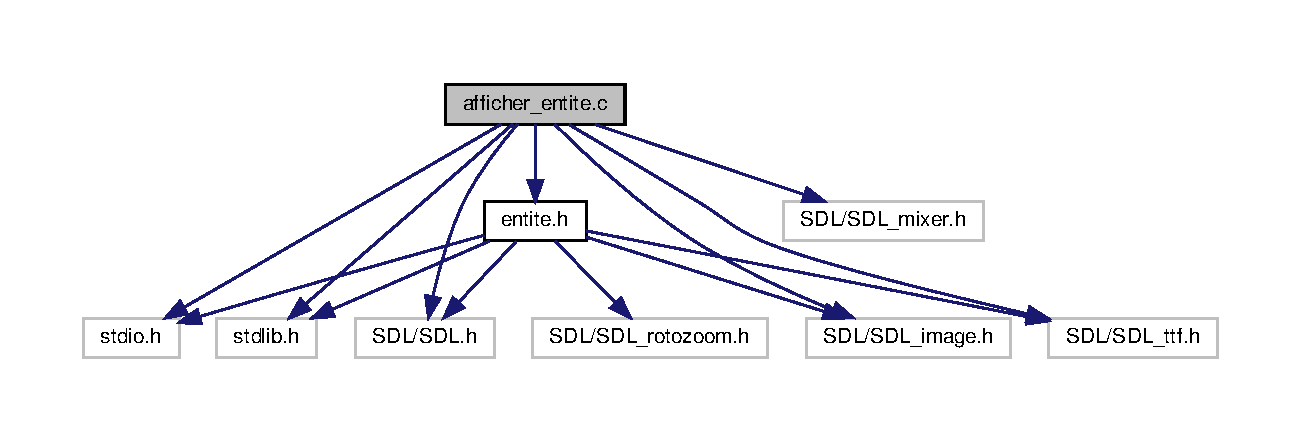
\includegraphics[width=350pt]{afficher__entite_8c__incl}
\end{center}
\end{figure}
\subsection*{Functions}
\begin{DoxyCompactItemize}
\item 
void \hyperlink{afficher__entite_8c_ae7d96b4436a6a7d64da6147dae6ebaea}{afficher\+\_\+entite\+\_\+secondaire} (\hyperlink{structent}{ent} $\ast$E, S\+D\+L\+\_\+\+Surface $\ast$ecran)
\begin{DoxyCompactList}\small\item\em afficher une entite secondaire. \end{DoxyCompactList}\end{DoxyCompactItemize}


\subsection{Function Documentation}
\mbox{\Hypertarget{afficher__entite_8c_ae7d96b4436a6a7d64da6147dae6ebaea}\label{afficher__entite_8c_ae7d96b4436a6a7d64da6147dae6ebaea}} 
\index{afficher\+\_\+entite.\+c@{afficher\+\_\+entite.\+c}!afficher\+\_\+entite\+\_\+secondaire@{afficher\+\_\+entite\+\_\+secondaire}}
\index{afficher\+\_\+entite\+\_\+secondaire@{afficher\+\_\+entite\+\_\+secondaire}!afficher\+\_\+entite.\+c@{afficher\+\_\+entite.\+c}}
\subsubsection{\texorpdfstring{afficher\+\_\+entite\+\_\+secondaire()}{afficher\_entite\_secondaire()}}
{\footnotesize\ttfamily void afficher\+\_\+entite\+\_\+secondaire (\begin{DoxyParamCaption}\item[{\hyperlink{structent}{ent} $\ast$}]{E,  }\item[{S\+D\+L\+\_\+\+Surface $\ast$}]{ecran }\end{DoxyParamCaption})}



afficher une entite secondaire. 

\begin{DoxyAuthor}{Author}
Boubakri Nawres 
\end{DoxyAuthor}

\begin{DoxyParams}{Parameters}
{\em E} & entite \\
\hline
{\em ecran} & l\textquotesingle{}ecran \\
\hline
\end{DoxyParams}
\begin{DoxyReturn}{Returns}
Nothing 
\end{DoxyReturn}

\hypertarget{anim__entite__droite_8c}{}\section{anim\+\_\+entite\+\_\+droite.\+c File Reference}
\label{anim__entite__droite_8c}\index{anim\+\_\+entite\+\_\+droite.\+c@{anim\+\_\+entite\+\_\+droite.\+c}}
{\ttfamily \#include $<$stdio.\+h$>$}\newline
{\ttfamily \#include $<$stdlib.\+h$>$}\newline
{\ttfamily \#include $<$math.\+h$>$}\newline
{\ttfamily \#include $<$string.\+h$>$}\newline
{\ttfamily \#include $<$S\+D\+L/\+S\+D\+L.\+h$>$}\newline
{\ttfamily \#include $<$S\+D\+L/\+S\+D\+L\+\_\+image.\+h$>$}\newline
{\ttfamily \#include $<$S\+D\+L/\+S\+D\+L\+\_\+ttf.\+h$>$}\newline
{\ttfamily \#include $<$S\+D\+L/\+S\+D\+L\+\_\+mixer.\+h$>$}\newline
{\ttfamily \#include $<$time.\+h$>$}\newline
{\ttfamily \#include \char`\"{}entite.\+h\char`\"{}}\newline
Include dependency graph for anim\+\_\+entite\+\_\+droite.\+c\+:
\nopagebreak
\begin{figure}[H]
\begin{center}
\leavevmode
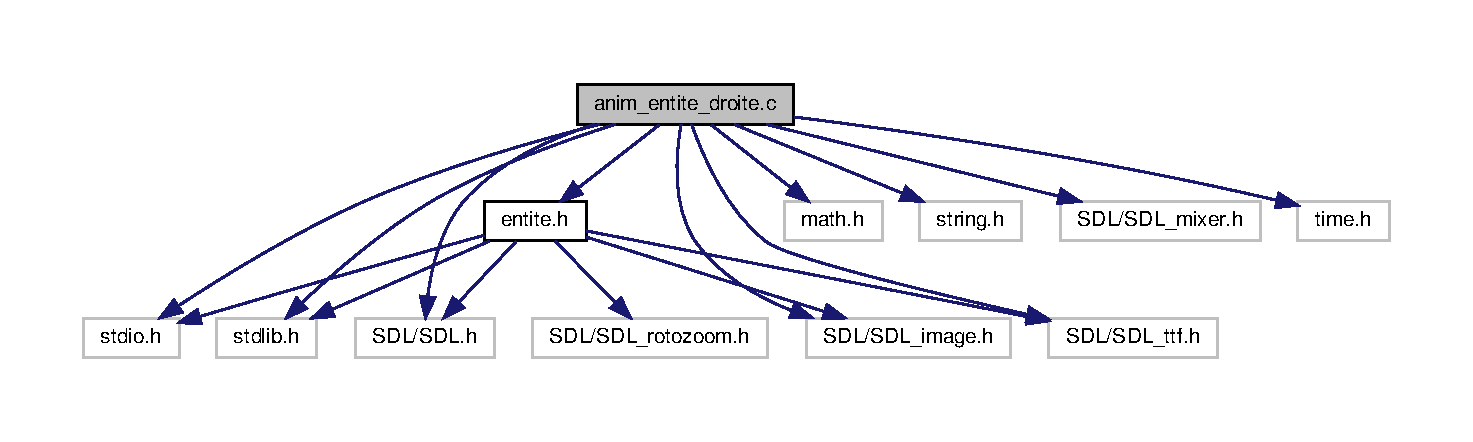
\includegraphics[width=350pt]{anim__entite__droite_8c__incl}
\end{center}
\end{figure}
\subsection*{Functions}
\begin{DoxyCompactItemize}
\item 
void \hyperlink{anim__entite__droite_8c_ab48cf68616e1e9e1db8c519cdb6c3282}{animation\+\_\+entite\+\_\+droite} (\hyperlink{structent}{ent} $\ast$E, S\+D\+L\+\_\+\+Rect rects\mbox{[}$\,$\mbox{]}, S\+D\+L\+\_\+\+Surface $\ast$screen, S\+D\+L\+\_\+\+Surface $\ast$Background, S\+D\+L\+\_\+\+Rect position\+Fond)
\begin{DoxyCompactList}\small\item\em animer l\textquotesingle{}entite . \end{DoxyCompactList}\end{DoxyCompactItemize}


\subsection{Function Documentation}
\mbox{\Hypertarget{anim__entite__droite_8c_ab48cf68616e1e9e1db8c519cdb6c3282}\label{anim__entite__droite_8c_ab48cf68616e1e9e1db8c519cdb6c3282}} 
\index{anim\+\_\+entite\+\_\+droite.\+c@{anim\+\_\+entite\+\_\+droite.\+c}!animation\+\_\+entite\+\_\+droite@{animation\+\_\+entite\+\_\+droite}}
\index{animation\+\_\+entite\+\_\+droite@{animation\+\_\+entite\+\_\+droite}!anim\+\_\+entite\+\_\+droite.\+c@{anim\+\_\+entite\+\_\+droite.\+c}}
\subsubsection{\texorpdfstring{animation\+\_\+entite\+\_\+droite()}{animation\_entite\_droite()}}
{\footnotesize\ttfamily void animation\+\_\+entite\+\_\+droite (\begin{DoxyParamCaption}\item[{\hyperlink{structent}{ent} $\ast$}]{E,  }\item[{S\+D\+L\+\_\+\+Rect}]{rects\mbox{[}$\,$\mbox{]},  }\item[{S\+D\+L\+\_\+\+Surface $\ast$}]{screen,  }\item[{S\+D\+L\+\_\+\+Surface $\ast$}]{Background,  }\item[{S\+D\+L\+\_\+\+Rect}]{position\+Fond }\end{DoxyParamCaption})}



animer l\textquotesingle{}entite . 

\begin{DoxyAuthor}{Author}
Boubakri Nawres 
\end{DoxyAuthor}

\begin{DoxyParams}{Parameters}
{\em E} & entite \\
\hline
{\em rects\mbox{[}$\,$\mbox{]}} & frame \\
\hline
{\em screen} & l\textquotesingle{}ecran \\
\hline
{\em Background} & \\
\hline
{\em position\+Fond} & \\
\hline
\end{DoxyParams}
\begin{DoxyReturn}{Returns}
Nothing 
\end{DoxyReturn}
Here is the caller graph for this function\+:
\nopagebreak
\begin{figure}[H]
\begin{center}
\leavevmode
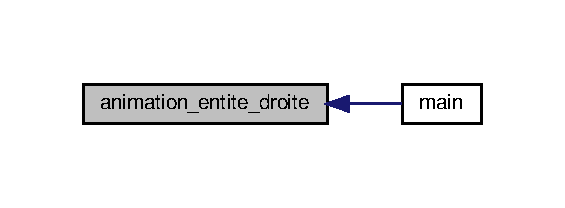
\includegraphics[width=271pt]{anim__entite__droite_8c_ab48cf68616e1e9e1db8c519cdb6c3282_icgraph}
\end{center}
\end{figure}

\hypertarget{animate__enemy_8c}{}\section{animate\+\_\+enemy.\+c File Reference}
\label{animate__enemy_8c}\index{animate\+\_\+enemy.\+c@{animate\+\_\+enemy.\+c}}
{\ttfamily \#include $<$stdio.\+h$>$}\newline
{\ttfamily \#include $<$stdlib.\+h$>$}\newline
{\ttfamily \#include $<$S\+D\+L/\+S\+D\+L.\+h$>$}\newline
{\ttfamily \#include $<$S\+D\+L/\+S\+D\+L\+\_\+image.\+h$>$}\newline
{\ttfamily \#include $<$S\+D\+L/\+S\+D\+L\+\_\+ttf.\+h$>$}\newline
{\ttfamily \#include \char`\"{}entite.\+h\char`\"{}}\newline
Include dependency graph for animate\+\_\+enemy.\+c\+:
\nopagebreak
\begin{figure}[H]
\begin{center}
\leavevmode
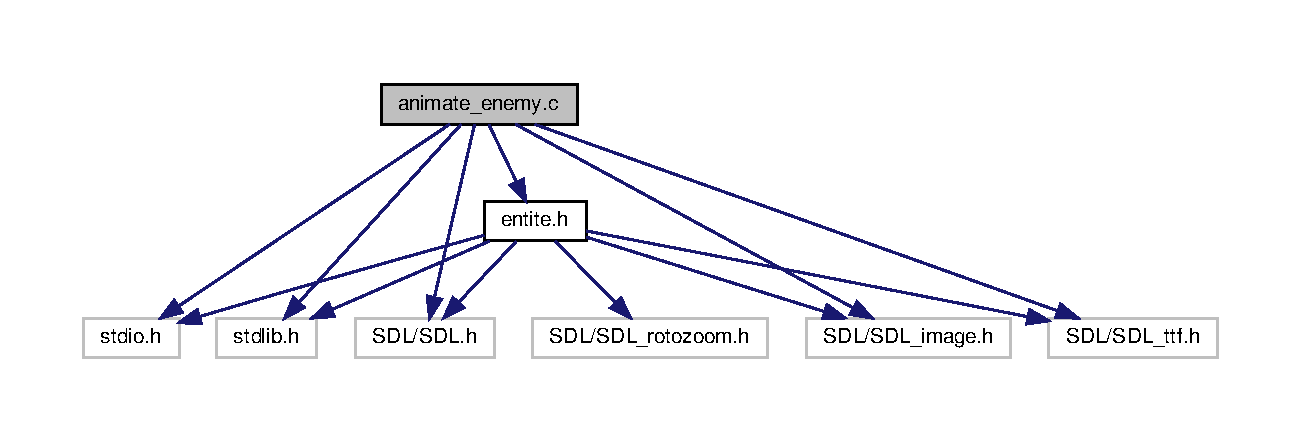
\includegraphics[width=350pt]{animate__enemy_8c__incl}
\end{center}
\end{figure}
\subsection*{Functions}
\begin{DoxyCompactItemize}
\item 
void \hyperlink{animate__enemy_8c_afd9d9848c9d6c8faa6a8fd46c79cdc0f}{animate\+Ennemi} (\hyperlink{structent}{ent} $\ast$E, S\+D\+L\+\_\+\+Rect rects\mbox{[}$\,$\mbox{]}, S\+D\+L\+\_\+\+Surface $\ast$screen, S\+D\+L\+\_\+\+Surface $\ast$Background, S\+D\+L\+\_\+\+Rect position\+Fond)
\begin{DoxyCompactList}\small\item\em animer une entite secondaire. \end{DoxyCompactList}\end{DoxyCompactItemize}


\subsection{Function Documentation}
\mbox{\Hypertarget{animate__enemy_8c_afd9d9848c9d6c8faa6a8fd46c79cdc0f}\label{animate__enemy_8c_afd9d9848c9d6c8faa6a8fd46c79cdc0f}} 
\index{animate\+\_\+enemy.\+c@{animate\+\_\+enemy.\+c}!animate\+Ennemi@{animate\+Ennemi}}
\index{animate\+Ennemi@{animate\+Ennemi}!animate\+\_\+enemy.\+c@{animate\+\_\+enemy.\+c}}
\subsubsection{\texorpdfstring{animate\+Ennemi()}{animateEnnemi()}}
{\footnotesize\ttfamily void animate\+Ennemi (\begin{DoxyParamCaption}\item[{\hyperlink{structent}{ent} $\ast$}]{E,  }\item[{S\+D\+L\+\_\+\+Rect}]{rects\mbox{[}$\,$\mbox{]},  }\item[{S\+D\+L\+\_\+\+Surface $\ast$}]{screen,  }\item[{S\+D\+L\+\_\+\+Surface $\ast$}]{Background,  }\item[{S\+D\+L\+\_\+\+Rect}]{position\+Fond }\end{DoxyParamCaption})}



animer une entite secondaire. 

\begin{DoxyAuthor}{Author}
Boubakri Nawres 
\end{DoxyAuthor}

\begin{DoxyParams}{Parameters}
{\em E} & entite \\
\hline
{\em screen} & l\textquotesingle{}ecran \\
\hline
{\em Background} & \\
\hline
{\em position\+Fond} & \\
\hline
\end{DoxyParams}
\begin{DoxyReturn}{Returns}
Nothing 
\end{DoxyReturn}
Here is the caller graph for this function\+:
\nopagebreak
\begin{figure}[H]
\begin{center}
\leavevmode
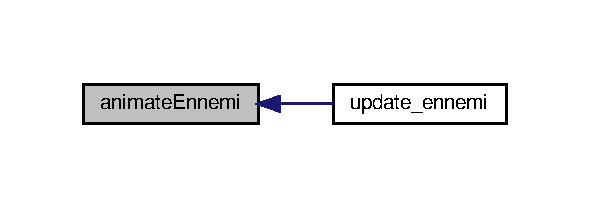
\includegraphics[width=283pt]{animate__enemy_8c_afd9d9848c9d6c8faa6a8fd46c79cdc0f_icgraph}
\end{center}
\end{figure}

\hypertarget{dep__va__x_8c}{}\section{dep\+\_\+va\+\_\+x.\+c File Reference}
\label{dep__va__x_8c}\index{dep\+\_\+va\+\_\+x.\+c@{dep\+\_\+va\+\_\+x.\+c}}
{\ttfamily \#include $<$stdio.\+h$>$}\newline
{\ttfamily \#include $<$stdlib.\+h$>$}\newline
{\ttfamily \#include $<$S\+D\+L/\+S\+D\+L.\+h$>$}\newline
{\ttfamily \#include $<$S\+D\+L/\+S\+D\+L\+\_\+image.\+h$>$}\newline
{\ttfamily \#include $<$S\+D\+L/\+S\+D\+L\+\_\+ttf.\+h$>$}\newline
{\ttfamily \#include \char`\"{}entite.\+h\char`\"{}}\newline
Include dependency graph for dep\+\_\+va\+\_\+x.\+c\+:
\nopagebreak
\begin{figure}[H]
\begin{center}
\leavevmode
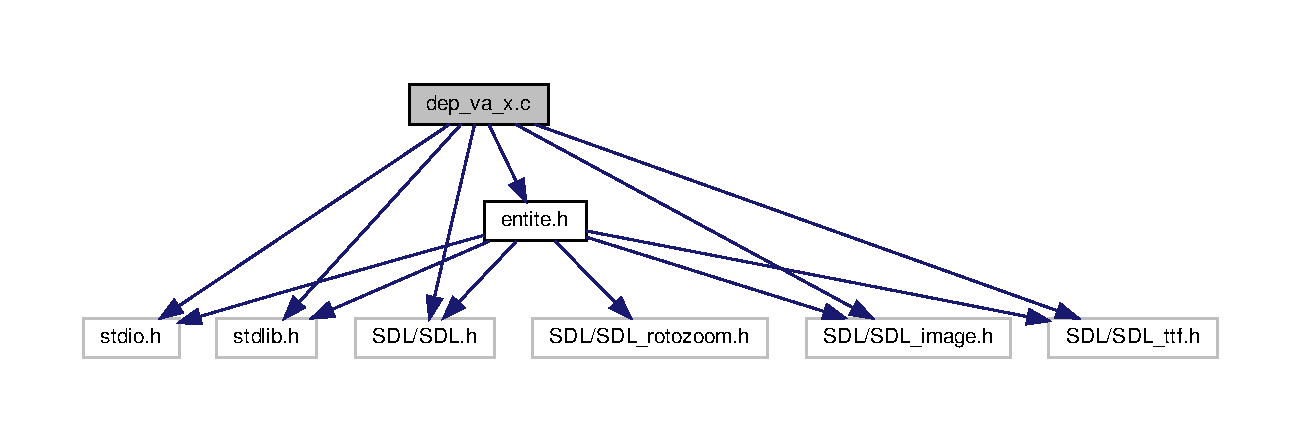
\includegraphics[width=350pt]{dep__va__x_8c__incl}
\end{center}
\end{figure}
\subsection*{Functions}
\begin{DoxyCompactItemize}
\item 
void \hyperlink{dep__va__x_8c_ad9f185c74df9373a6037cba7d6350123}{enemy\+\_\+va\+\_\+x} (\hyperlink{structent}{ent} $\ast$E)
\begin{DoxyCompactList}\small\item\em movement va et vient sur x . \end{DoxyCompactList}\end{DoxyCompactItemize}


\subsection{Function Documentation}
\mbox{\Hypertarget{dep__va__x_8c_ad9f185c74df9373a6037cba7d6350123}\label{dep__va__x_8c_ad9f185c74df9373a6037cba7d6350123}} 
\index{dep\+\_\+va\+\_\+x.\+c@{dep\+\_\+va\+\_\+x.\+c}!enemy\+\_\+va\+\_\+x@{enemy\+\_\+va\+\_\+x}}
\index{enemy\+\_\+va\+\_\+x@{enemy\+\_\+va\+\_\+x}!dep\+\_\+va\+\_\+x.\+c@{dep\+\_\+va\+\_\+x.\+c}}
\subsubsection{\texorpdfstring{enemy\+\_\+va\+\_\+x()}{enemy\_va\_x()}}
{\footnotesize\ttfamily void enemy\+\_\+va\+\_\+x (\begin{DoxyParamCaption}\item[{\hyperlink{structent}{ent} $\ast$}]{E }\end{DoxyParamCaption})}



movement va et vient sur x . 

\begin{DoxyAuthor}{Author}
Boubakri Nawres 
\end{DoxyAuthor}

\begin{DoxyParams}{Parameters}
{\em E} & entite\\
\hline
\end{DoxyParams}
\begin{DoxyReturn}{Returns}
Nothing 
\end{DoxyReturn}
Here is the call graph for this function\+:
\nopagebreak
\begin{figure}[H]
\begin{center}
\leavevmode
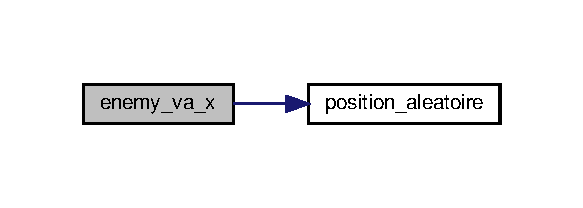
\includegraphics[width=280pt]{dep__va__x_8c_ad9f185c74df9373a6037cba7d6350123_cgraph}
\end{center}
\end{figure}
Here is the caller graph for this function\+:
\nopagebreak
\begin{figure}[H]
\begin{center}
\leavevmode
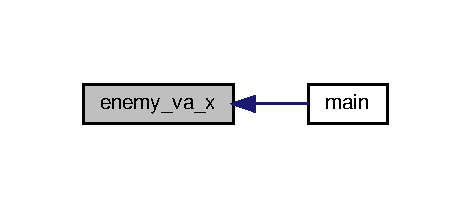
\includegraphics[width=226pt]{dep__va__x_8c_ad9f185c74df9373a6037cba7d6350123_icgraph}
\end{center}
\end{figure}

\hypertarget{free__enemy_8c}{}\section{free\+\_\+enemy.\+c File Reference}
\label{free__enemy_8c}\index{free\+\_\+enemy.\+c@{free\+\_\+enemy.\+c}}
{\ttfamily \#include $<$stdio.\+h$>$}\newline
{\ttfamily \#include $<$stdlib.\+h$>$}\newline
{\ttfamily \#include $<$S\+D\+L/\+S\+D\+L.\+h$>$}\newline
{\ttfamily \#include $<$S\+D\+L/\+S\+D\+L\+\_\+image.\+h$>$}\newline
{\ttfamily \#include $<$S\+D\+L/\+S\+D\+L\+\_\+ttf.\+h$>$}\newline
{\ttfamily \#include \char`\"{}entite.\+h\char`\"{}}\newline
Include dependency graph for free\+\_\+enemy.\+c\+:
\nopagebreak
\begin{figure}[H]
\begin{center}
\leavevmode
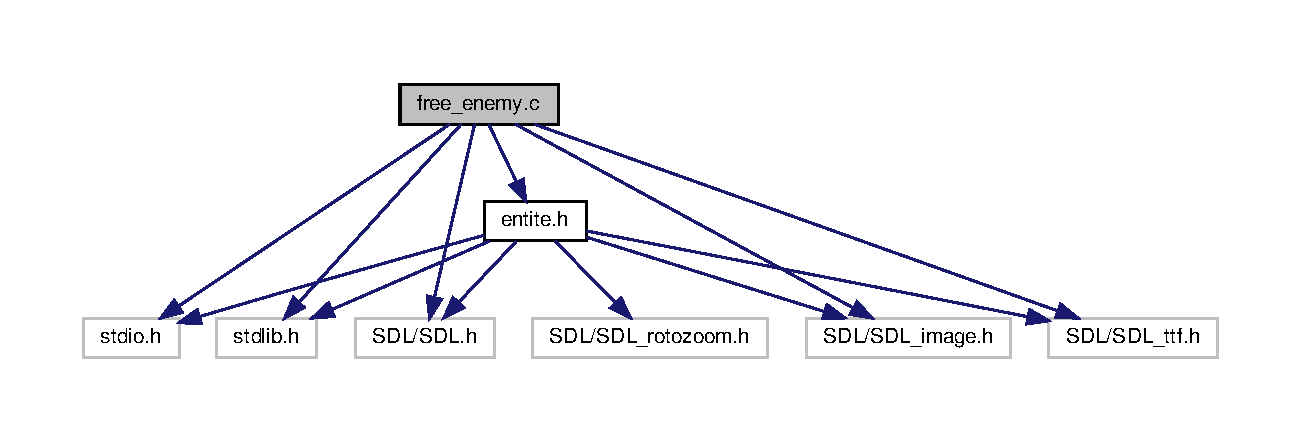
\includegraphics[width=350pt]{free__enemy_8c__incl}
\end{center}
\end{figure}
\subsection*{Functions}
\begin{DoxyCompactItemize}
\item 
void \hyperlink{free__enemy_8c_a9bbe908fbe8cf252565c5a6058c5086c}{free\+Ennemi} (\hyperlink{structent}{ent} $\ast$E)
\begin{DoxyCompactList}\small\item\em free sufrace. \end{DoxyCompactList}\end{DoxyCompactItemize}


\subsection{Function Documentation}
\mbox{\Hypertarget{free__enemy_8c_a9bbe908fbe8cf252565c5a6058c5086c}\label{free__enemy_8c_a9bbe908fbe8cf252565c5a6058c5086c}} 
\index{free\+\_\+enemy.\+c@{free\+\_\+enemy.\+c}!free\+Ennemi@{free\+Ennemi}}
\index{free\+Ennemi@{free\+Ennemi}!free\+\_\+enemy.\+c@{free\+\_\+enemy.\+c}}
\subsubsection{\texorpdfstring{free\+Ennemi()}{freeEnnemi()}}
{\footnotesize\ttfamily void free\+Ennemi (\begin{DoxyParamCaption}\item[{\hyperlink{structent}{ent} $\ast$}]{E }\end{DoxyParamCaption})}



free sufrace. 

\begin{DoxyAuthor}{Author}
Boubakri Nawres 
\end{DoxyAuthor}

\begin{DoxyParams}{Parameters}
{\em E} & entite\\
\hline
\end{DoxyParams}
\begin{DoxyReturn}{Returns}
Nothing 
\end{DoxyReturn}

\hypertarget{init__entite_8c}{}\section{init\+\_\+entite.\+c File Reference}
\label{init__entite_8c}\index{init\+\_\+entite.\+c@{init\+\_\+entite.\+c}}
{\ttfamily \#include $<$stdio.\+h$>$}\newline
{\ttfamily \#include $<$stdlib.\+h$>$}\newline
{\ttfamily \#include $<$math.\+h$>$}\newline
{\ttfamily \#include $<$string.\+h$>$}\newline
{\ttfamily \#include $<$S\+D\+L/\+S\+D\+L.\+h$>$}\newline
{\ttfamily \#include $<$S\+D\+L/\+S\+D\+L\+\_\+image.\+h$>$}\newline
{\ttfamily \#include $<$S\+D\+L/\+S\+D\+L\+\_\+ttf.\+h$>$}\newline
{\ttfamily \#include $<$S\+D\+L/\+S\+D\+L\+\_\+mixer.\+h$>$}\newline
{\ttfamily \#include $<$time.\+h$>$}\newline
{\ttfamily \#include \char`\"{}entite.\+h\char`\"{}}\newline
Include dependency graph for init\+\_\+entite.\+c\+:
\nopagebreak
\begin{figure}[H]
\begin{center}
\leavevmode
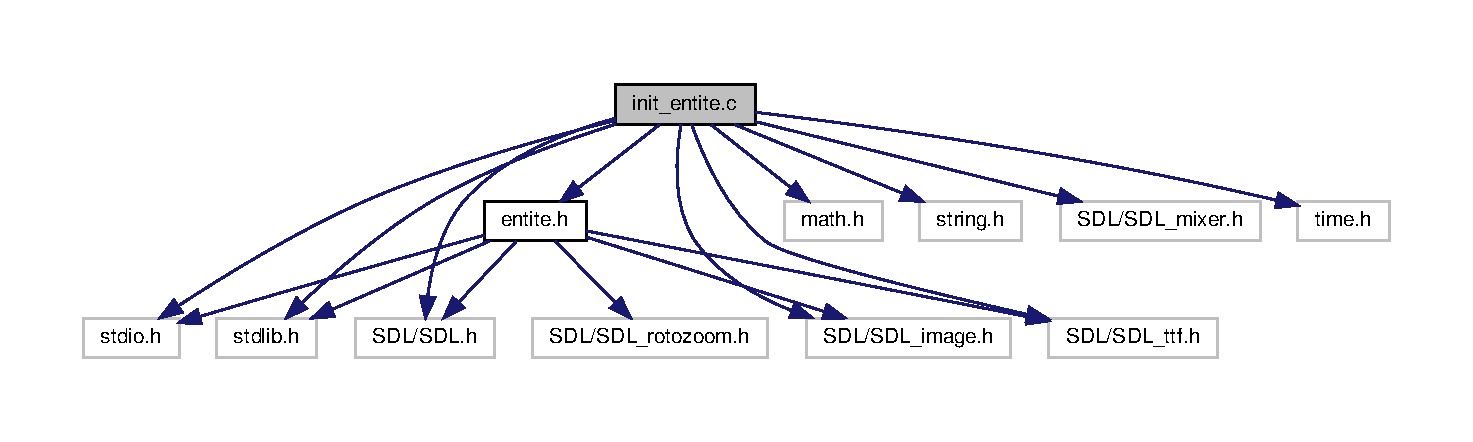
\includegraphics[width=350pt]{init__entite_8c__incl}
\end{center}
\end{figure}
\subsection*{Functions}
\begin{DoxyCompactItemize}
\item 
void \hyperlink{init__entite_8c_a9acc5655f404d5728a0deb4ec36665b9}{initialiser\+\_\+entite} (\hyperlink{structent}{ent} E\mbox{[}$\,$\mbox{]}, int n)
\begin{DoxyCompactList}\small\item\em initialiser l\textquotesingle{}entite . \end{DoxyCompactList}\end{DoxyCompactItemize}


\subsection{Function Documentation}
\mbox{\Hypertarget{init__entite_8c_a9acc5655f404d5728a0deb4ec36665b9}\label{init__entite_8c_a9acc5655f404d5728a0deb4ec36665b9}} 
\index{init\+\_\+entite.\+c@{init\+\_\+entite.\+c}!initialiser\+\_\+entite@{initialiser\+\_\+entite}}
\index{initialiser\+\_\+entite@{initialiser\+\_\+entite}!init\+\_\+entite.\+c@{init\+\_\+entite.\+c}}
\subsubsection{\texorpdfstring{initialiser\+\_\+entite()}{initialiser\_entite()}}
{\footnotesize\ttfamily void initialiser\+\_\+entite (\begin{DoxyParamCaption}\item[{\hyperlink{structent}{ent}}]{E\mbox{[}$\,$\mbox{]},  }\item[{int}]{n }\end{DoxyParamCaption})}



initialiser l\textquotesingle{}entite . 

\begin{DoxyAuthor}{Author}
Boubakri Nawres 
\end{DoxyAuthor}

\begin{DoxyParams}{Parameters}
{\em E\mbox{[}$\,$\mbox{]}} & entite \\
\hline
{\em n} & nombre d\textquotesingle{}entite\\
\hline
\end{DoxyParams}
\begin{DoxyReturn}{Returns}
Nothing 
\end{DoxyReturn}
Here is the caller graph for this function\+:
\nopagebreak
\begin{figure}[H]
\begin{center}
\leavevmode
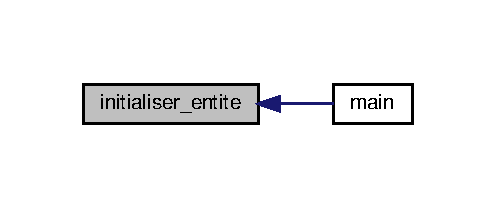
\includegraphics[width=238pt]{init__entite_8c_a9acc5655f404d5728a0deb4ec36665b9_icgraph}
\end{center}
\end{figure}

\hypertarget{main_8c}{}\section{main.\+c File Reference}
\label{main_8c}\index{main.\+c@{main.\+c}}


Testing Program.  


{\ttfamily \#include $<$stdio.\+h$>$}\newline
{\ttfamily \#include $<$stdlib.\+h$>$}\newline
{\ttfamily \#include $<$S\+D\+L/\+S\+D\+L.\+h$>$}\newline
{\ttfamily \#include $<$S\+D\+L/\+S\+D\+L\+\_\+image.\+h$>$}\newline
{\ttfamily \#include \char`\"{}fonction.\+h\char`\"{}}\newline
Include dependency graph for main.\+c\+:
\nopagebreak
\begin{figure}[H]
\begin{center}
\leavevmode
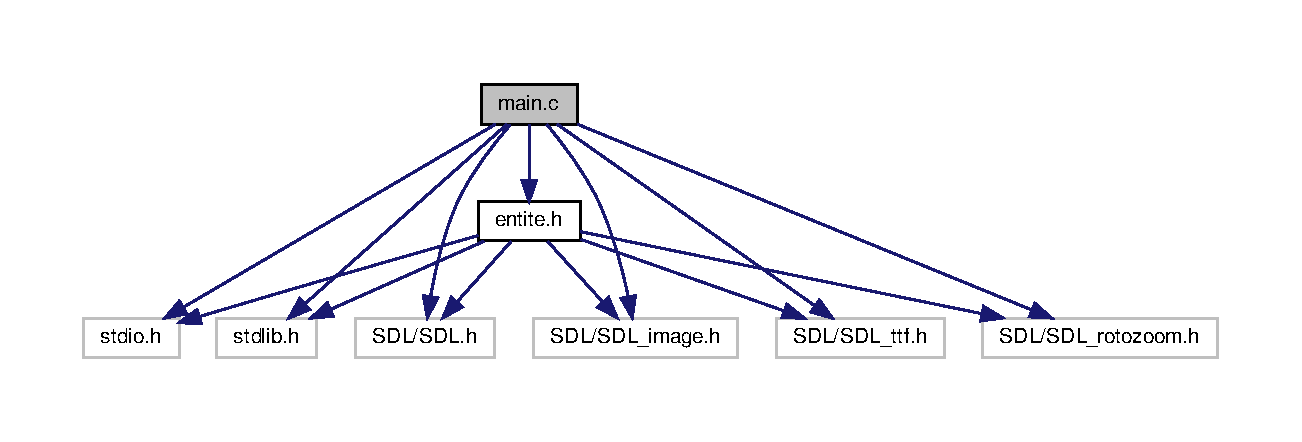
\includegraphics[width=350pt]{main_8c__incl}
\end{center}
\end{figure}
\subsection*{Functions}
\begin{DoxyCompactItemize}
\item 
\mbox{\Hypertarget{main_8c_ae66f6b31b5ad750f1fe042a706a4e3d4}\label{main_8c_ae66f6b31b5ad750f1fe042a706a4e3d4}} 
int {\bfseries main} ()
\end{DoxyCompactItemize}


\subsection{Detailed Description}
Testing Program. 

\begin{DoxyAuthor}{Author}
A\+N\+O\+UN Y\+O\+U\+S\+S\+EF 
\end{DoxyAuthor}
\begin{DoxyVersion}{Version}
0.\+1 
\end{DoxyVersion}
\begin{DoxyDate}{Date}
Apr 01, 2019
\end{DoxyDate}
Testing program for collision bounding box 
\hypertarget{move__enemy_8c}{}\section{move\+\_\+enemy.\+c File Reference}
\label{move__enemy_8c}\index{move\+\_\+enemy.\+c@{move\+\_\+enemy.\+c}}
{\ttfamily \#include $<$stdio.\+h$>$}\newline
{\ttfamily \#include $<$stdlib.\+h$>$}\newline
{\ttfamily \#include $<$S\+D\+L/\+S\+D\+L.\+h$>$}\newline
{\ttfamily \#include $<$S\+D\+L/\+S\+D\+L\+\_\+image.\+h$>$}\newline
{\ttfamily \#include $<$S\+D\+L/\+S\+D\+L\+\_\+ttf.\+h$>$}\newline
{\ttfamily \#include \char`\"{}entite.\+h\char`\"{}}\newline
Include dependency graph for move\+\_\+enemy.\+c\+:
\nopagebreak
\begin{figure}[H]
\begin{center}
\leavevmode
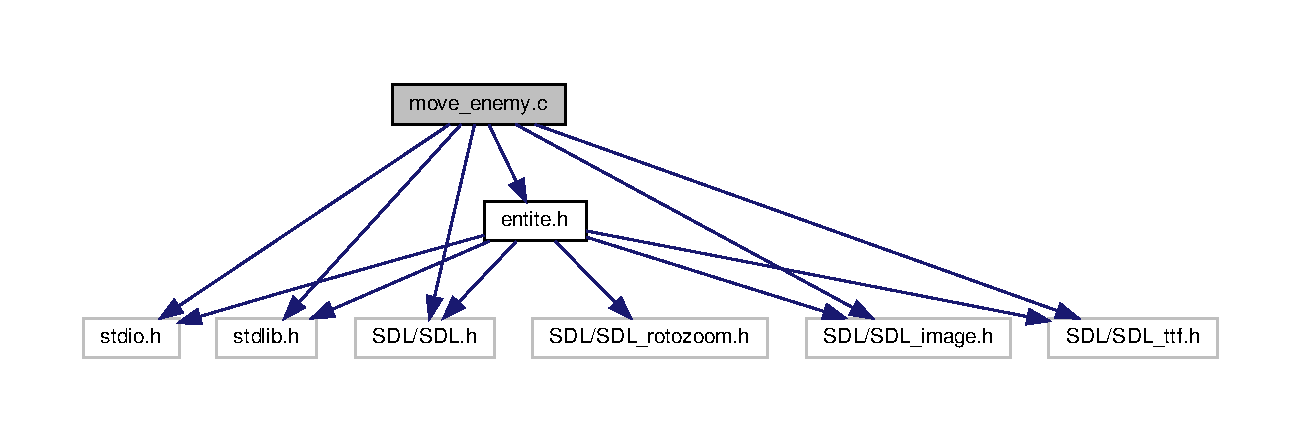
\includegraphics[width=350pt]{move__enemy_8c__incl}
\end{center}
\end{figure}
\subsection*{Functions}
\begin{DoxyCompactItemize}
\item 
void \hyperlink{move__enemy_8c_a0076f6ab2615806da91d06a2541dc722}{move\+\_\+ennemi} (\hyperlink{structent}{ent} $\ast$E, S\+D\+L\+\_\+\+Rect pos\+Hero)
\begin{DoxyCompactList}\small\item\em afficher une entite secondaire. \end{DoxyCompactList}\end{DoxyCompactItemize}


\subsection{Function Documentation}
\mbox{\Hypertarget{move__enemy_8c_a0076f6ab2615806da91d06a2541dc722}\label{move__enemy_8c_a0076f6ab2615806da91d06a2541dc722}} 
\index{move\+\_\+enemy.\+c@{move\+\_\+enemy.\+c}!move\+\_\+ennemi@{move\+\_\+ennemi}}
\index{move\+\_\+ennemi@{move\+\_\+ennemi}!move\+\_\+enemy.\+c@{move\+\_\+enemy.\+c}}
\subsubsection{\texorpdfstring{move\+\_\+ennemi()}{move\_ennemi()}}
{\footnotesize\ttfamily void move\+\_\+ennemi (\begin{DoxyParamCaption}\item[{\hyperlink{structent}{ent} $\ast$}]{E,  }\item[{S\+D\+L\+\_\+\+Rect}]{pos\+Hero }\end{DoxyParamCaption})}



afficher une entite secondaire. 

\begin{DoxyAuthor}{Author}
Boubakri Nawres 
\end{DoxyAuthor}

\begin{DoxyParams}{Parameters}
{\em E} & entite \\
\hline
{\em pos\+Hero} & position de l\textquotesingle{}hero \\
\hline
\end{DoxyParams}
\begin{DoxyReturn}{Returns}
Nothing 
\end{DoxyReturn}
Here is the caller graph for this function\+:
\nopagebreak
\begin{figure}[H]
\begin{center}
\leavevmode
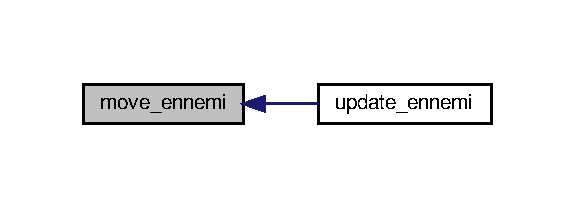
\includegraphics[width=276pt]{move__enemy_8c_a0076f6ab2615806da91d06a2541dc722_icgraph}
\end{center}
\end{figure}

\hypertarget{pos__alea_8c}{}\section{pos\+\_\+alea.\+c File Reference}
\label{pos__alea_8c}\index{pos\+\_\+alea.\+c@{pos\+\_\+alea.\+c}}
{\ttfamily \#include $<$stdio.\+h$>$}\newline
{\ttfamily \#include $<$stdlib.\+h$>$}\newline
{\ttfamily \#include $<$math.\+h$>$}\newline
{\ttfamily \#include $<$string.\+h$>$}\newline
{\ttfamily \#include $<$S\+D\+L/\+S\+D\+L.\+h$>$}\newline
{\ttfamily \#include $<$S\+D\+L/\+S\+D\+L\+\_\+image.\+h$>$}\newline
{\ttfamily \#include $<$S\+D\+L/\+S\+D\+L\+\_\+ttf.\+h$>$}\newline
{\ttfamily \#include $<$S\+D\+L/\+S\+D\+L\+\_\+mixer.\+h$>$}\newline
{\ttfamily \#include $<$time.\+h$>$}\newline
{\ttfamily \#include \char`\"{}entite.\+h\char`\"{}}\newline
Include dependency graph for pos\+\_\+alea.\+c\+:
\nopagebreak
\begin{figure}[H]
\begin{center}
\leavevmode
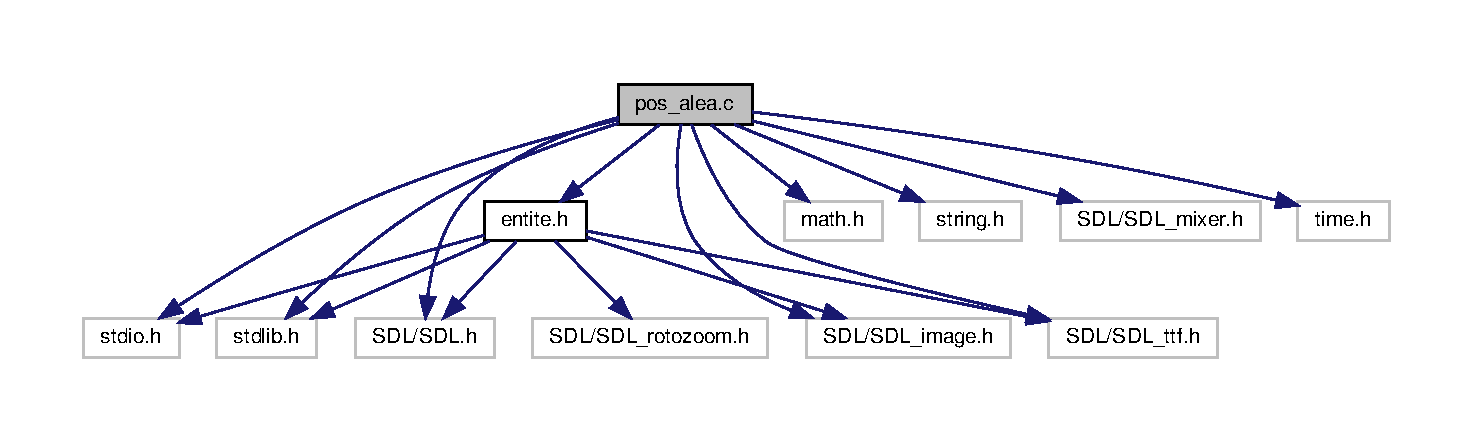
\includegraphics[width=350pt]{pos__alea_8c__incl}
\end{center}
\end{figure}
\subsection*{Functions}
\begin{DoxyCompactItemize}
\item 
int \hyperlink{pos__alea_8c_a3b66d6d37682e944f1aa89d1727dbf6d}{position\+\_\+aleatoire} (int positionmax, int positionmin)
\begin{DoxyCompactList}\small\item\em donner une positon aleatoire . \end{DoxyCompactList}\end{DoxyCompactItemize}


\subsection{Function Documentation}
\mbox{\Hypertarget{pos__alea_8c_a3b66d6d37682e944f1aa89d1727dbf6d}\label{pos__alea_8c_a3b66d6d37682e944f1aa89d1727dbf6d}} 
\index{pos\+\_\+alea.\+c@{pos\+\_\+alea.\+c}!position\+\_\+aleatoire@{position\+\_\+aleatoire}}
\index{position\+\_\+aleatoire@{position\+\_\+aleatoire}!pos\+\_\+alea.\+c@{pos\+\_\+alea.\+c}}
\subsubsection{\texorpdfstring{position\+\_\+aleatoire()}{position\_aleatoire()}}
{\footnotesize\ttfamily int position\+\_\+aleatoire (\begin{DoxyParamCaption}\item[{int}]{positionmax,  }\item[{int}]{positionmin }\end{DoxyParamCaption})}



donner une positon aleatoire . 

\begin{DoxyAuthor}{Author}
Boubakri Nawres 
\end{DoxyAuthor}

\begin{DoxyParams}{Parameters}
{\em positionmax} & \\
\hline
{\em positionmin} & \\
\hline
\end{DoxyParams}
\begin{DoxyReturn}{Returns}
int 
\end{DoxyReturn}
Here is the caller graph for this function\+:
\nopagebreak
\begin{figure}[H]
\begin{center}
\leavevmode
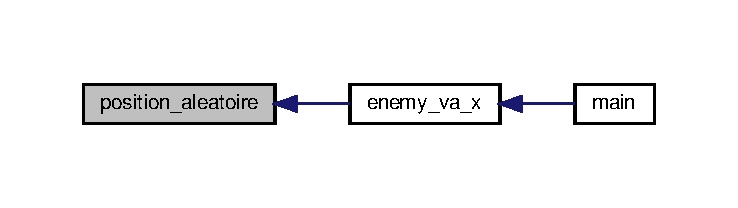
\includegraphics[width=350pt]{pos__alea_8c_a3b66d6d37682e944f1aa89d1727dbf6d_icgraph}
\end{center}
\end{figure}

\hypertarget{roto_8c}{}\section{roto.\+c File Reference}
\label{roto_8c}\index{roto.\+c@{roto.\+c}}
{\ttfamily \#include \char`\"{}entite.\+h\char`\"{}}\newline
{\ttfamily \#include $<$stdio.\+h$>$}\newline
{\ttfamily \#include \char`\"{}S\+D\+L/\+S\+D\+L.\+h\char`\"{}}\newline
{\ttfamily \#include \char`\"{}S\+D\+L/\+S\+D\+L\+\_\+image.\+h\char`\"{}}\newline
{\ttfamily \#include \char`\"{}S\+D\+L/\+S\+D\+L\+\_\+mixer.\+h\char`\"{}}\newline
{\ttfamily \#include $<$time.\+h$>$}\newline
{\ttfamily \#include $<$S\+D\+L/\+S\+D\+L\+\_\+rotozoom.\+h$>$}\newline
Include dependency graph for roto.\+c\+:
\nopagebreak
\begin{figure}[H]
\begin{center}
\leavevmode
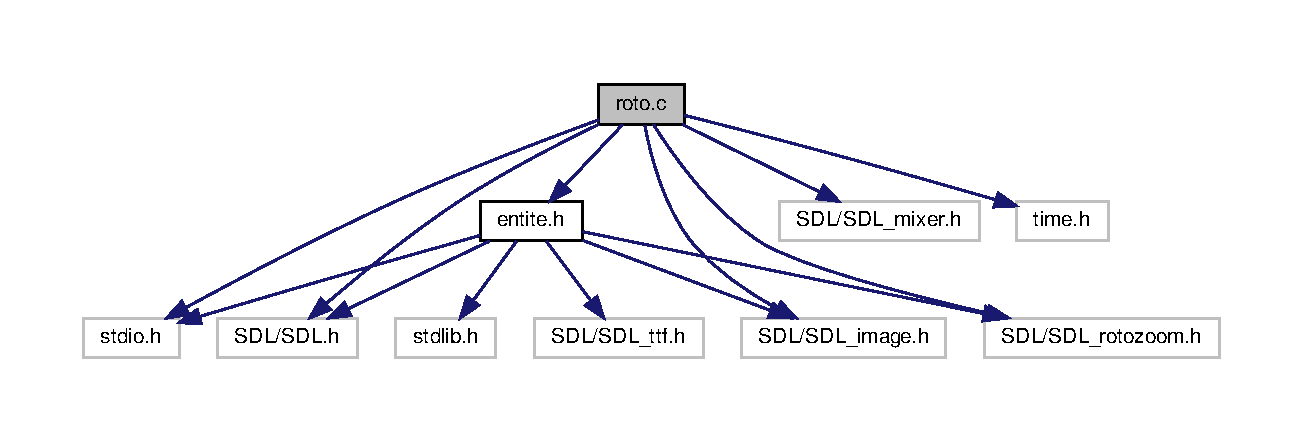
\includegraphics[width=350pt]{roto_8c__incl}
\end{center}
\end{figure}
\subsection*{Functions}
\begin{DoxyCompactItemize}
\item 
void \hyperlink{roto_8c_a1b1138caa5218b229c7baea8cd4215c6}{rotation\+\_\+enemy} (\hyperlink{structent}{ent} E, S\+D\+L\+\_\+\+Surface $\ast$ecran, S\+D\+L\+\_\+\+Surface $\ast$backg, S\+D\+L\+\_\+\+Rect position\+Fond)
\begin{DoxyCompactList}\small\item\em rotation et zoom de l\textquotesingle{}entite . \end{DoxyCompactList}\end{DoxyCompactItemize}


\subsection{Function Documentation}
\mbox{\Hypertarget{roto_8c_a1b1138caa5218b229c7baea8cd4215c6}\label{roto_8c_a1b1138caa5218b229c7baea8cd4215c6}} 
\index{roto.\+c@{roto.\+c}!rotation\+\_\+enemy@{rotation\+\_\+enemy}}
\index{rotation\+\_\+enemy@{rotation\+\_\+enemy}!roto.\+c@{roto.\+c}}
\subsubsection{\texorpdfstring{rotation\+\_\+enemy()}{rotation\_enemy()}}
{\footnotesize\ttfamily void rotation\+\_\+enemy (\begin{DoxyParamCaption}\item[{\hyperlink{structent}{ent}}]{E,  }\item[{S\+D\+L\+\_\+\+Surface $\ast$}]{ecran,  }\item[{S\+D\+L\+\_\+\+Surface $\ast$}]{backg,  }\item[{S\+D\+L\+\_\+\+Rect}]{position\+Fond }\end{DoxyParamCaption})}



rotation et zoom de l\textquotesingle{}entite . 

\begin{DoxyAuthor}{Author}
Boubakri Nawres 
\end{DoxyAuthor}

\begin{DoxyParams}{Parameters}
{\em E} & entite \\
\hline
{\em ecran} & l\textquotesingle{}ecran \\
\hline
{\em backg} & background \\
\hline
{\em position\+Fond} & \\
\hline
\end{DoxyParams}
\begin{DoxyReturn}{Returns}
Nothing 
\end{DoxyReturn}

\hypertarget{update__enemy_8c}{}\section{update\+\_\+enemy.\+c File Reference}
\label{update__enemy_8c}\index{update\+\_\+enemy.\+c@{update\+\_\+enemy.\+c}}
{\ttfamily \#include $<$stdio.\+h$>$}\newline
{\ttfamily \#include $<$stdlib.\+h$>$}\newline
{\ttfamily \#include $<$S\+D\+L/\+S\+D\+L.\+h$>$}\newline
{\ttfamily \#include $<$S\+D\+L/\+S\+D\+L\+\_\+image.\+h$>$}\newline
{\ttfamily \#include $<$S\+D\+L/\+S\+D\+L\+\_\+ttf.\+h$>$}\newline
{\ttfamily \#include \char`\"{}entite.\+h\char`\"{}}\newline
Include dependency graph for update\+\_\+enemy.\+c\+:
\nopagebreak
\begin{figure}[H]
\begin{center}
\leavevmode
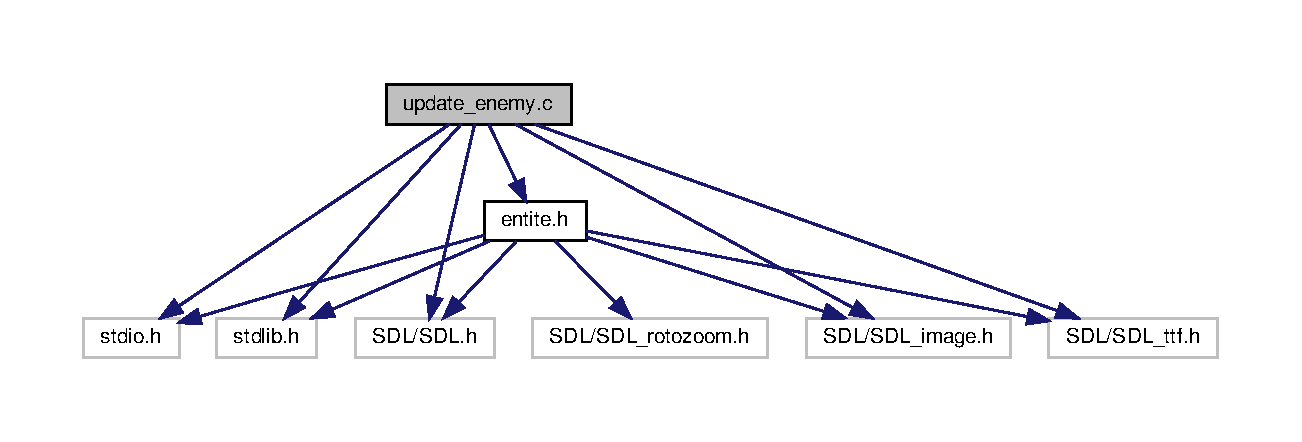
\includegraphics[width=350pt]{update__enemy_8c__incl}
\end{center}
\end{figure}
\subsection*{Functions}
\begin{DoxyCompactItemize}
\item 
void \hyperlink{update__enemy_8c_a13259e08f6729794f8cf68fb895cee95}{update\+\_\+ennemi} (\hyperlink{structent}{ent} $\ast$E, S\+D\+L\+\_\+\+Rect pos\+Hero, S\+D\+L\+\_\+\+Rect rects\mbox{[}$\,$\mbox{]}, S\+D\+L\+\_\+\+Surface $\ast$screen, S\+D\+L\+\_\+\+Surface $\ast$Background, S\+D\+L\+\_\+\+Rect position\+Fond)
\begin{DoxyCompactList}\small\item\em mise a jour de l\textquotesingle{}ennemi \end{DoxyCompactList}\end{DoxyCompactItemize}


\subsection{Function Documentation}
\mbox{\Hypertarget{update__enemy_8c_a13259e08f6729794f8cf68fb895cee95}\label{update__enemy_8c_a13259e08f6729794f8cf68fb895cee95}} 
\index{update\+\_\+enemy.\+c@{update\+\_\+enemy.\+c}!update\+\_\+ennemi@{update\+\_\+ennemi}}
\index{update\+\_\+ennemi@{update\+\_\+ennemi}!update\+\_\+enemy.\+c@{update\+\_\+enemy.\+c}}
\subsubsection{\texorpdfstring{update\+\_\+ennemi()}{update\_ennemi()}}
{\footnotesize\ttfamily void update\+\_\+ennemi (\begin{DoxyParamCaption}\item[{\hyperlink{structent}{ent} $\ast$}]{E,  }\item[{S\+D\+L\+\_\+\+Rect}]{pos\+Hero,  }\item[{S\+D\+L\+\_\+\+Rect}]{rects\mbox{[}$\,$\mbox{]},  }\item[{S\+D\+L\+\_\+\+Surface $\ast$}]{screen,  }\item[{S\+D\+L\+\_\+\+Surface $\ast$}]{Background,  }\item[{S\+D\+L\+\_\+\+Rect}]{position\+Fond }\end{DoxyParamCaption})}



mise a jour de l\textquotesingle{}ennemi 

\begin{DoxyAuthor}{Author}
Boubakri Nawres 
\end{DoxyAuthor}

\begin{DoxyParams}{Parameters}
{\em E} & entite \\
\hline
{\em pos\+Hero} & position de l\textquotesingle{}hero \\
\hline
{\em rects\mbox{[}$\,$\mbox{]}} & \\
\hline
{\em screen} & \\
\hline
{\em Background} & \\
\hline
{\em position\+Fond} & \\
\hline
\end{DoxyParams}
\begin{DoxyReturn}{Returns}
Nothing 
\end{DoxyReturn}
Here is the call graph for this function\+:
\nopagebreak
\begin{figure}[H]
\begin{center}
\leavevmode
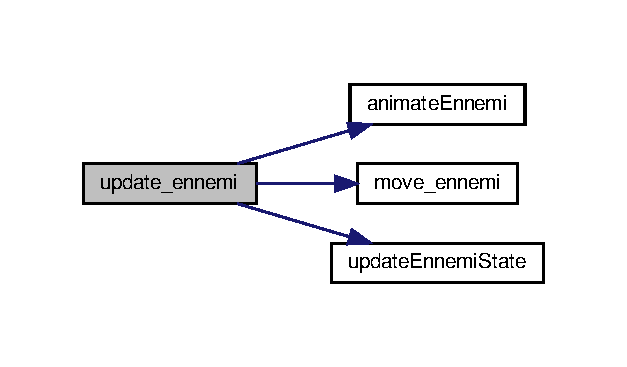
\includegraphics[width=301pt]{update__enemy_8c_a13259e08f6729794f8cf68fb895cee95_cgraph}
\end{center}
\end{figure}

\hypertarget{update__enemy__state_8c}{}\section{update\+\_\+enemy\+\_\+state.\+c File Reference}
\label{update__enemy__state_8c}\index{update\+\_\+enemy\+\_\+state.\+c@{update\+\_\+enemy\+\_\+state.\+c}}
{\ttfamily \#include $<$stdio.\+h$>$}\newline
{\ttfamily \#include $<$stdlib.\+h$>$}\newline
{\ttfamily \#include $<$S\+D\+L/\+S\+D\+L.\+h$>$}\newline
{\ttfamily \#include $<$S\+D\+L/\+S\+D\+L\+\_\+image.\+h$>$}\newline
{\ttfamily \#include $<$S\+D\+L/\+S\+D\+L\+\_\+ttf.\+h$>$}\newline
{\ttfamily \#include \char`\"{}entite.\+h\char`\"{}}\newline
Include dependency graph for update\+\_\+enemy\+\_\+state.\+c\+:
\nopagebreak
\begin{figure}[H]
\begin{center}
\leavevmode
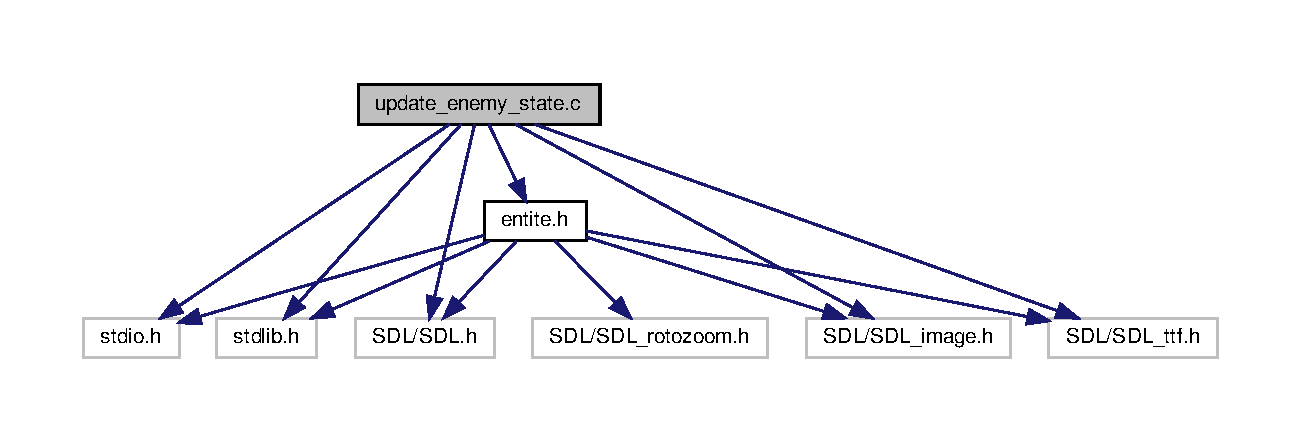
\includegraphics[width=350pt]{update__enemy__state_8c__incl}
\end{center}
\end{figure}
\subsection*{Functions}
\begin{DoxyCompactItemize}
\item 
void \hyperlink{update__enemy__state_8c_a553c154d7bb37e20d867366b66799803}{update\+Ennemi\+State} (\hyperlink{structent}{ent} $\ast$E, int dist\+EH)
\begin{DoxyCompactList}\small\item\em update enemy state. \end{DoxyCompactList}\end{DoxyCompactItemize}


\subsection{Function Documentation}
\mbox{\Hypertarget{update__enemy__state_8c_a553c154d7bb37e20d867366b66799803}\label{update__enemy__state_8c_a553c154d7bb37e20d867366b66799803}} 
\index{update\+\_\+enemy\+\_\+state.\+c@{update\+\_\+enemy\+\_\+state.\+c}!update\+Ennemi\+State@{update\+Ennemi\+State}}
\index{update\+Ennemi\+State@{update\+Ennemi\+State}!update\+\_\+enemy\+\_\+state.\+c@{update\+\_\+enemy\+\_\+state.\+c}}
\subsubsection{\texorpdfstring{update\+Ennemi\+State()}{updateEnnemiState()}}
{\footnotesize\ttfamily void update\+Ennemi\+State (\begin{DoxyParamCaption}\item[{\hyperlink{structent}{ent} $\ast$}]{E,  }\item[{int}]{dist\+EH }\end{DoxyParamCaption})}



update enemy state. 

\begin{DoxyAuthor}{Author}
Boubakri Nawres 
\end{DoxyAuthor}

\begin{DoxyParams}{Parameters}
{\em E} & entite \\
\hline
{\em dist\+EH} & distance enemy\+\_\+hero \\
\hline
\end{DoxyParams}
\begin{DoxyReturn}{Returns}
Nothing 
\end{DoxyReturn}
Here is the caller graph for this function\+:
\nopagebreak
\begin{figure}[H]
\begin{center}
\leavevmode
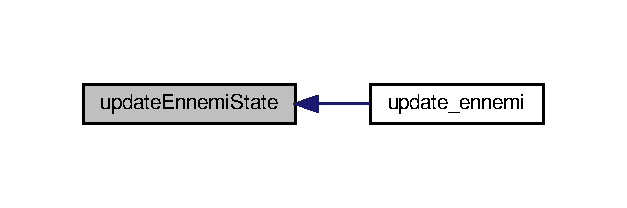
\includegraphics[width=301pt]{update__enemy__state_8c_a553c154d7bb37e20d867366b66799803_icgraph}
\end{center}
\end{figure}

%--- End generated contents ---

% Index
\backmatter
\newpage
\phantomsection
\clearemptydoublepage
\addcontentsline{toc}{chapter}{Index}
\printindex

\end{document}
